%%%%%%%%%%%%%%%%%%%%%%%%%%%%%%%%%%%%%%%%%
% Beamer Presentation
% LaTeX Template
% Version 1.0 (10/11/12)
%
% This template has been downloaded from:
% http://www.LaTeXTemplates.com
%
% License:
% CC BY-NC-SA 3.0 (http://creativecommons.org/licenses/by-nc-sa/3.0/)
%
%%%%%%%%%%%%%%%%%%%%%%%%%%%%%%%%%%%%%%%%%

%----------------------------------------------------------------------------------------
%	PACKAGES AND THEMES
%----------------------------------------------------------------------------------------

\documentclass{beamer}

\mode<presentation> {

% The Beamer class comes with a number of default slide themes
% which change the colors and layouts of slides. Below this is a list
% of all the themes, uncomment each in turn to see what they look like.

%\usetheme{default}
%\usetheme{AnnArbor}
%\usetheme{Antibes}
%\usetheme{Bergen}
%\usetheme{Berkeley}
%\usetheme{Berlin}
%\usetheme{Boadilla}
%\usetheme{CambridgeUS}
%\usetheme{Copenhagen}
%\usetheme{Darmstadt}
%\usetheme{Dresden}
%\usetheme{Frankfurt}
%\usetheme{Goettingen}
%\usetheme{Hannover}
%\usetheme{Ilmenau}
%\usetheme{JuanLesPins}
%\usetheme{Luebeck}
\usetheme{Madrid}
%\usetheme{Malmoe}
%\usetheme{Marburg}
%\usetheme{Montpellier}
%\usetheme{PaloAlto}
%\usetheme{Pittsburgh}
%\usetheme{Rochester}
%\usetheme{Singapore}
%\usetheme{Szeged}
%\usetheme{Warsaw}

% As well as themes, the Beamer class has a number of color themes
% for any slide theme. Uncomment each of these in turn to see how it
% changes the colors of your current slide theme.

%\usecolortheme{albatross}
%\usecolortheme{beaver}
%\usecolortheme{beetle}
%\usecolortheme{crane}
%\usecolortheme{dolphin}
%\usecolortheme{dove}
%\usecolortheme{fly}
%\usecolortheme{lily}
%\usecolortheme{orchid}
%\usecolortheme{rose}
%\usecolortheme{seagull}
%\usecolortheme{seahorse}
%\usecolortheme{whale}
%\usecolortheme{wolverine}

%\setbeamertemplate{footline} % To remove the footer line in all slides uncomment this line
%\setbeamertemplate{footline}[page number] % To replace the footer line in all slides with a simple slide count uncomment this line

%\setbeamertemplate{navigation symbols}{} % To remove the navigation symbols from the bottom of all slides uncomment this line
}

\usepackage{graphicx} % Allows including images


\begin{document}

\section{Multi-Output Prediction Model}

\begin{frame}{Bayesian additive regression tree (BART)}
\begin{itemize}
\item Nonparametric prediction tool
\item Ensemble of 'weak learners' that leads to robust out-of-sample predictions
\item Dynamically learns important predictors via a sparsity inducing prior
%\item Excels when $x$ is high in dimension, with relatively few important predictors
\end{itemize}

Mathematically, a BART model looks like:

\begin{align*}
Y_i &\sim N(\mu_i, \sigma^2)\\
\mu_i &= \sum_{t=1}^T \sum_{l \in L_t}\psi_{lt}I(x_i \leadsto (t,l))
\end{align*}

$I(x_i \leadsto (t,l)) = 1$ if $x_i$ falls into node ($t,l$) of tree $t$; 0 otherwise. 

\end{frame}

\begin{frame}{Shared Forest}
\begin{itemize}
\item An extension of BART for multivariate responses
\item Correlation between responses is utilized via shared tree structures
\item Variables that predict $Y_1$ are likely the same variables that predict $Y_2$ (though the nature of the relationship may be different!)
\item Information sharing $\Rightarrow$ better predictions for $Y_1$ \textit{and} $Y_2$ 
\end{itemize}
\end{frame}



\section{Simulation Study} 


\subsection{Binary/Continuous} 

\begin{frame}{1 binary, 1 continuous }
\begin{align}
Y_i &\sim N(\mu_i, \sigma^2_i) \\
\delta_i &\sim Bernoulli(\pi_i)
\end{align}

\begin{itemize}
\item $\begin{pmatrix}\mu_i \\ \pi_i \end{pmatrix}$ modeled jointly using a shared forest model

$$\begin{pmatrix}\mu_i \\ \Phi(\pi_i) \end{pmatrix} = 
\begin{pmatrix}\sum_{t=1}^T \sum_{l \in L_t}\psi_{lt}I(x_i \leadsto (t,l)) \\ \sum_{t=1}^T \sum_{l \in L_t}\theta_{lt}I(x_i \leadsto (t,l)) \end{pmatrix} $$
\item Likelihood involves two dimensional response: $\{Y_i, \delta_i\}_{i = 1}^N$
\end{itemize}
\end{frame}


\begin{frame}{Simulation Study }{Setup}
We run 100 simulations. In each:
\begin{itemize}
\item $n_{train} = 500$, $n_{test} = 500$
\item We set the number of covariates to P = 150. 
\item $x_1, \hdots, x_{150} \sim Unif(0,1)$
\item True underlying means based on a modification of the ``Friedman function"
\begin{align*}
y_i &= 10 \sin (\pi x_{1i} x_{2i}) + 20(x_{3i} - 0.5)^2 + 10x_{4i} + 5x_{5i} +
\epsilon_i^Y\\
\delta_i &= \begin{cases}1 &\text{ if}5 \sin (\pi x_{1i} x_{2i}) + 25(x_{3i} - 0.5)^2 + 5x_{4i} + 10x_{5i} +
\epsilon_i^{\delta} > 0 \\
                          0 & \text{ otherwise}\end{cases}
\end{align*}

where $(\epsilon_i^Y, \epsilon_i^{\delta}) \overset{iid}{\sim} N(0,1)$

\end{itemize}



\end{frame}

\begin{frame}{1 binary, 1 continuous }
Two quantities may be of interest for prediction
\begin{enumerate}
\item $E(\delta^*, y^* \mid x)$, where $^*$ indicates those observations come from a test / hold-out sample
  \begin{itemize}
    \item[ex)] Predict salary of individual, conditional on cellular traits $x_i$
    \item[ex)] Predict gender of individual, conditional on cellular traits $x_i$
  \end{itemize}
\item $E(y^* \mid \delta)$
  \begin{itemize}
    \item[ex)] Predict mean salary of females (avg. across traits observed for females)
  \end{itemize}
\end{enumerate}
\end{frame}


\begin{frame}{Predicting Individual $Y^*$ }
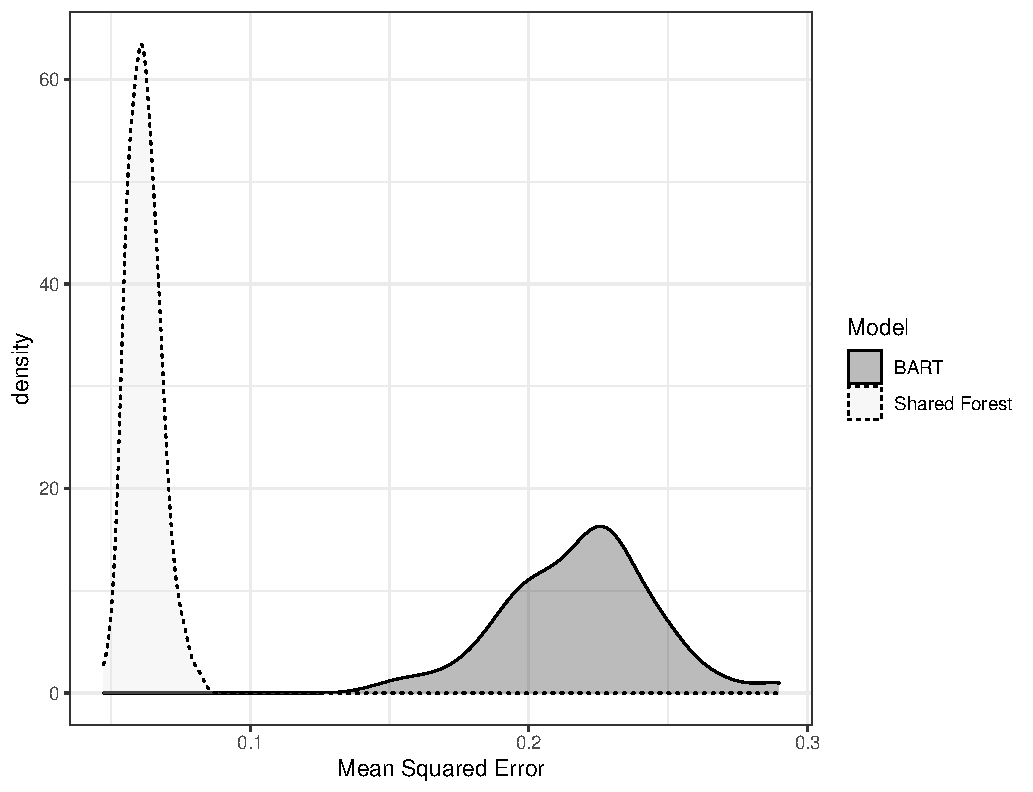
\includegraphics[width = .9\linewidth]{continuous_sim_results_ind_y.pdf}
\end{frame}

\begin{frame}{Predicting Individual $\delta*$}
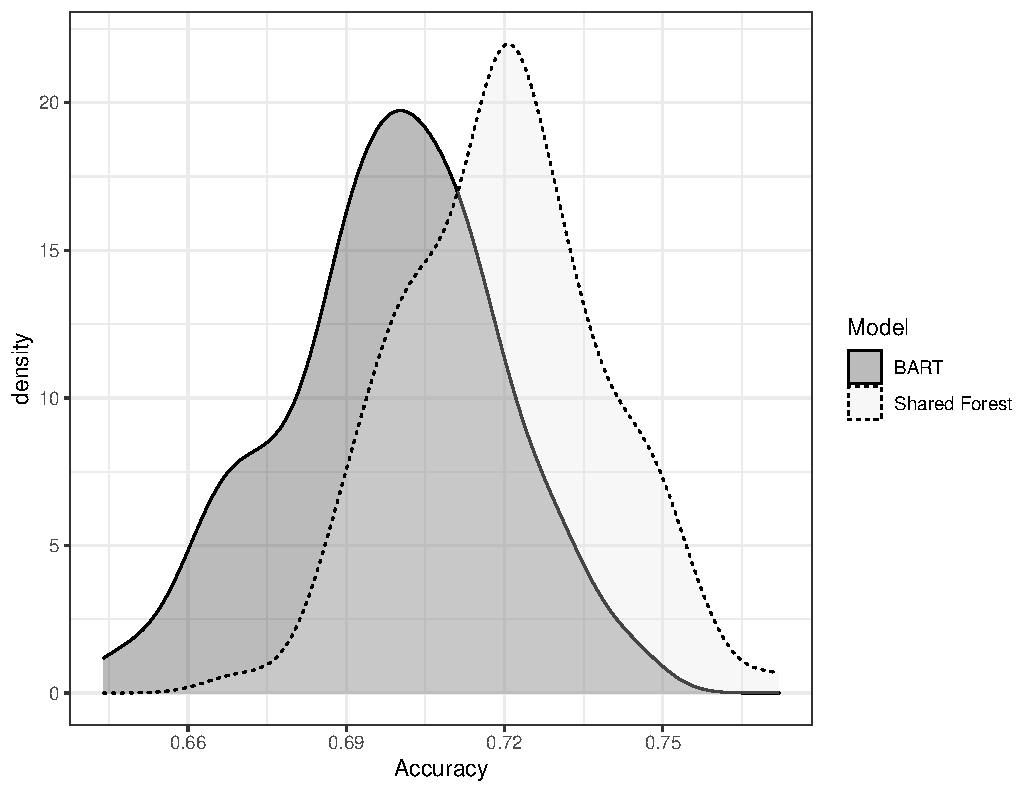
\includegraphics[width = .9\linewidth]{continuous_sim_results_ind_delta.pdf}
\end{frame}


\begin{frame}{Predicting $E(Y^* \mid \delta^*)$ }
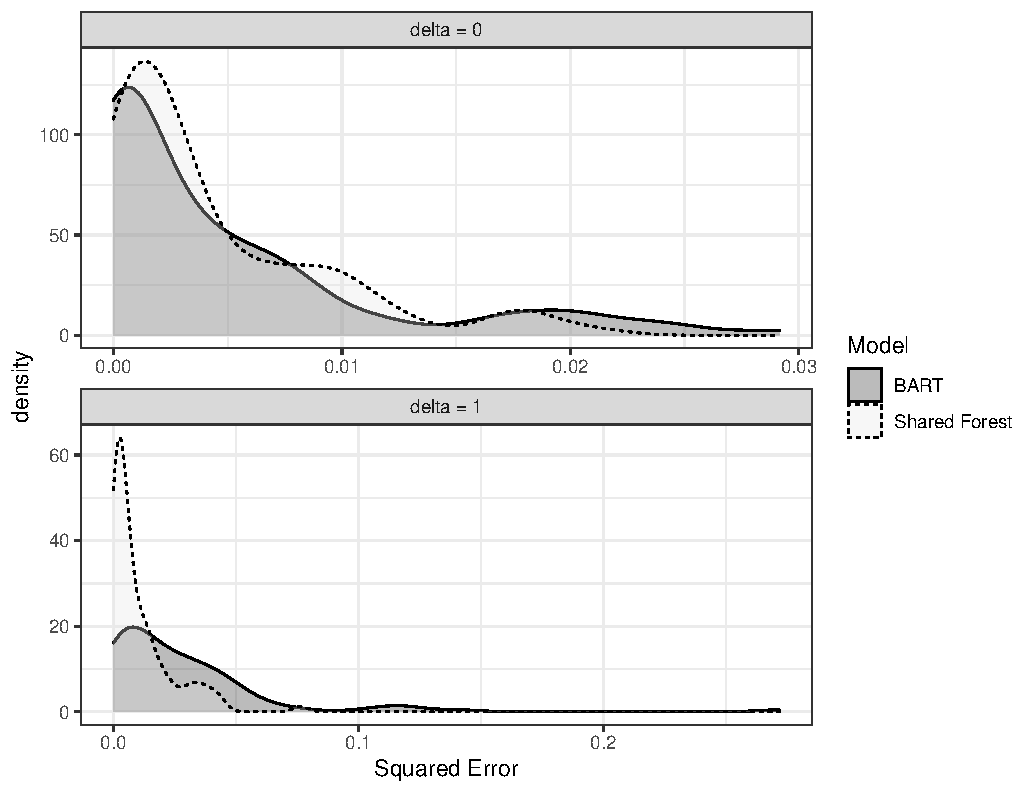
\includegraphics[width = .9\linewidth]{continuous_sim_results.pdf}
\end{frame}

\begin{frame}{Predicting $E(Y^* \mid \delta^*)$ }

% latex table generated in R 4.0.5 by xtable 1.8-4 package
% Tue Mar  1 10:17:05 2022
\begin{table}[ht]
\centering
\begin{tabular}{rlrrr}
  \hline
$\delta$ & Model & MSE & L\_bound & U\_bound \\ 
  \hline
0 & BART & 0.004875 & 0.000004 & 0.023207 \\ 
  0 & Shared Forest & 0.004330 & 0.000007 & 0.017697 \\ 
  1 & BART & 0.028464 & 0.000042 & 0.119264 \\ 
  1 & Shared Forest & 0.010399 & 0.000011 & 0.041591 \\ 
   \hline
\end{tabular}
\caption{\label{tab:mse} Mean of the squared errors (across simulations) comparing the true $E(Y^* \mid \delta^*)$ to the estimated $\hat{E}(Y^* \mid \hat{\delta})$.}
\end{table}

\end{frame}

\subsection{Binary/Binary} 

\begin{frame}{2 binary responses}
The model structure is the same as described before; however, the likelihood reflects that:

\begin{align}
\delta_{1i} &\sim Bernoulli(\pi_{1i}) \\
\delta_{2i} &\sim Bernoulli(\pi_{2i})
\end{align}

As before, the tree structures will be built using information shared between $\delta_1$ and $\delta_2$, while the location parameters are estimated separately. 

\end{frame}


\begin{frame}{2 binary responses}

In this context, we are interested in predicting $P(\delta^*_2=1 \mid \delta^*_1)$.
\begin{itemize}
\item[ex)] Probability a randomly selected female is employed. \\($\delta_1$ = gender, $\delta_2$ = employment)
\end{itemize}
We measure model performance by looking at the squared errors comparing the true population (conditional) means to the estimated. 

\end{frame}

\begin{frame}{Predicting $E(\delta_2^* \mid \delta_1^*)$ }
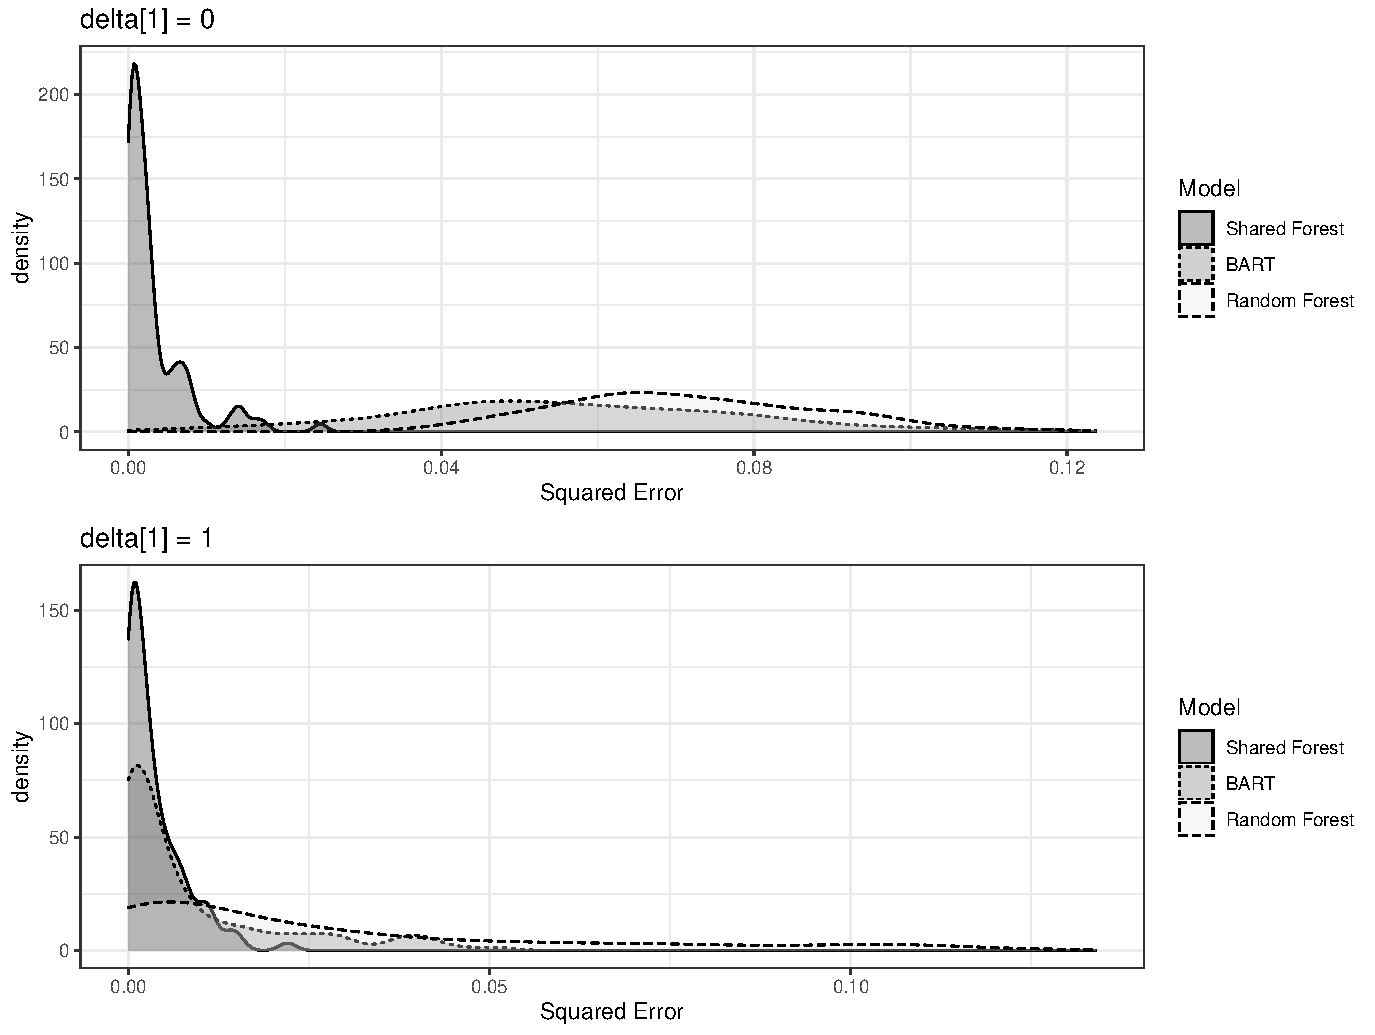
\includegraphics[width = .9\linewidth]{binary_sim_results.pdf}
\end{frame}

\end{document}